%%%%%%%%%%%%%%%%%%%%%%%%%%%%%%%%%%%%%%%%%%%%%%%%%%%%%%%%%
\chapter{Basic Components}
To work with practical electrical circuits, we need to familiarize ourselves with some common electric components. This section covers perfect wires, switches, resistors, and voltage and current sources. In particular, we'll examine simplified models of these components. Keep in mind, our goal is to make a model of the world that is correct enough to be useful and simple enough to be understandable.

\BI{Make your model as simple as possible, but no more. - Attributed to Albert Einstein (paraphrased).}

\section{Perfect wires}
A \emph{perfect} wire provides no resistance to the flow of electricity. Perfect wires don't actually exist, but many wires have little enough resistance that this resistance can be ignored \footnote{And even when it can't, we can lump into a resistor and locate it that resistor at one spot in the wire. Resistors will be covered later in this chapter.}.\par
On an electrical network diagram (a circuit diagram), a line represents a perfect wire.

\begin{figure}[H]
\begin{center}
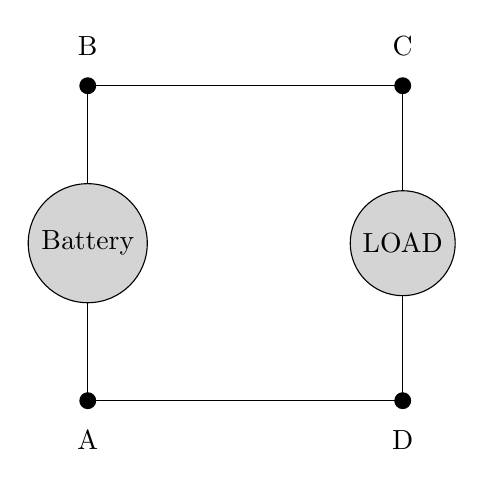
\begin{tikzpicture}
\draw (0,0)--(0,2) node[circle, draw=black,radius=0.25cm, fill={rgb:black,1;white,5}] {Battery}
--(0,4)--(4,4)--(4,2) node[circle, draw=black,radius=0.25cm, fill={rgb:black,1;white,5}] {LOAD}
--(4,0)--cycle;
\filldraw (4,0) circle[radius=1 mm]; \draw node at (4,-.5) {D};
\filldraw (4,4) circle[radius=1 mm]; \draw node at (4,4.5) {C};
\filldraw (0,4) circle[radius=1 mm]; \draw node at (0,4.5) {B};
\filldraw (0,0) circle[radius=1 mm]; \draw node at (0,-.5) {A};
\end{tikzpicture}
\label{F:2BL}
\end{center}
\end{figure}

For example, the network edge from B to C as drawn in Figure~\ref{F:2BL} represents a perfect wire because it was drawn as a line.
\par
\noindent
\begin{itemize}
\item \textbf{Observation:} If a perfect wire connects two nodes, these nodes will be at the same potential (voltage) and behave as one node.\footnote{You can also decide to treat a collection of nodes together, sometimes called a supernode), but then this supernode wouldn't have a unique voltage.} 
\item \textbf{Observation:} The length of a perfect wire does not matter. We'll usually draw whichever length makes the diagram most readable.
\item \textbf{Observation:} When wires cross, a dot indicates a connection. A lack of dot indicates no connection.
\end{itemize}
%%%%%%%%%%%%%%%%%%%%%%%%%%%%%%%%%%%%%%%%%%%%%%%%%%%%%%%%%%%%%%%%%%%
\section{Switches}
A perfect switch provides a break in the wire when \emph{open} and acts as a perfect wire when \emph{closed}. Figure~\ref{F:2BLa} shows a battery connected to a load via a switch.

\begin{figure}[H]
\begin{center}
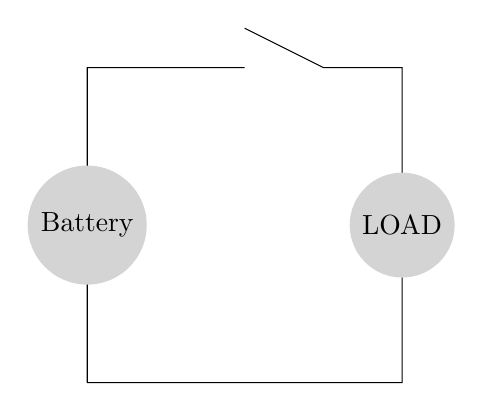
\begin{tikzpicture}
\draw (0,0) node(A){}
--(0,2) node[circle, radius=0.25cm, fill={rgb:black,1;white,5}] {Battery}
--(0,4)--(2,4) (2,4.5)--(3,4)--(4,4)
--(4,2) node[circle, radius=0.25cm, fill={rgb:black,1;white,5}] {LOAD}
--(4,0)
--(0,0);
\end{tikzpicture}
\caption{Battery connected to a load}
\label{F:2BLa}
\end{center}
\end{figure}

When the switch is open, the circuit has three nodes, labeled A, B and C as shown in Figure~\ref{F:2BLb}:

\begin{figure}[H]
\begin{center}
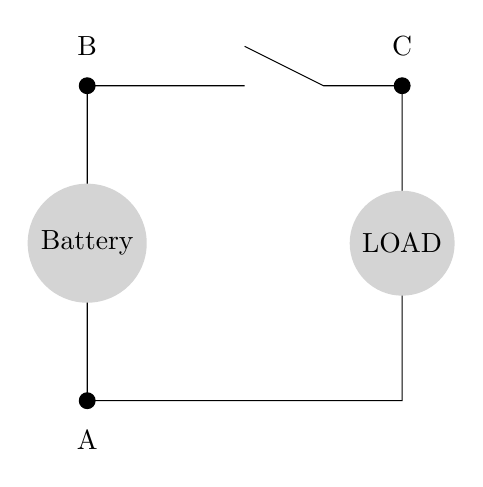
\begin{tikzpicture}
\draw (0,0) node(A){}
--(0,2) node[circle, radius=0.25cm, fill={rgb:black,1;white,5}] {Battery}
--(0,4)--(2,4) (2,4.5)--(3,4)--(4,4)
--(4,2) node[circle, radius=0.25cm, fill={rgb:black,1;white,5}] {LOAD}
--(4,0)--(0,0);
\filldraw (0,0) circle[radius=1 mm]; \draw node at (0,-.5) {A};
\filldraw (0,4) circle[radius=1 mm]; \draw node at (0,4.5) {B};
\filldraw (4,4) circle[radius=1 mm]; \draw node at (4,4.5) {C};
\end{tikzpicture}
\caption{Battery connected to a load with nodes indicated.}
\label{F:2BLb}
\end{center}
\end{figure}

When the switch is closed, the network has only two nodes. Nodes B and C become the same node, because they are connected with a perfect wire.\par


Many homes have three-way switches. The national electric code requires them for stairwells and other situations. A three-way switch allows one to turn off the stairwell light from the top or bottom of the staircase.
\par
Figure~\ref{F:23W} shows how such a switch might operate. The blue wire is the ground wire. We'll discuss that wire and its purpose later.
\par
\begin{figure}[H]
\begin{center}
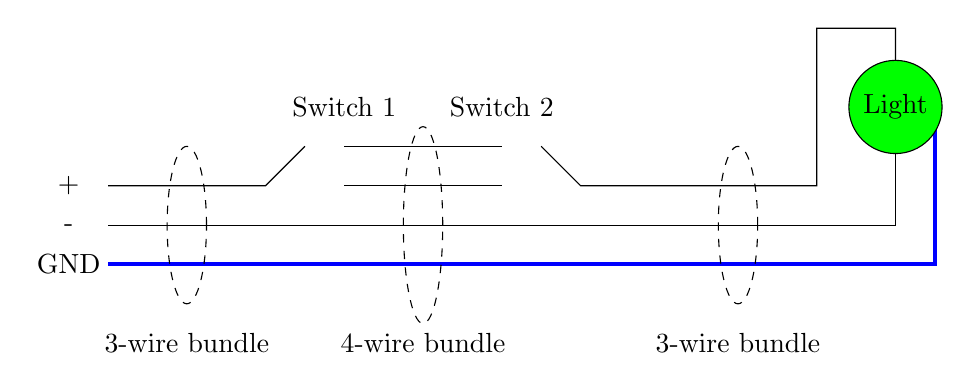
\begin{tikzpicture}
\draw [draw=blue, line width=0.5mm] (0,0) --(10.5,0)--(10.5,2) node(A){};
\draw (0,.5)--(10,0.5)--(10,2);
\draw (0,1)--(2,1)--(2.5,1.5);
\draw (3,1.5)--(5,1.5);
\draw (3,1)--(5,1);
\draw (5.5,1.5)--(6,1)--(9,1)--(9,3)--(10,3)--(10,2) node[circle,radius=.5cm,fill=green,draw=black](L) {Light};
\node at (3,2) {Switch 1};
\node at (5,2) {Switch 2};
\node at (1,-1) {3-wire bundle};
\node at (4,-1) {4-wire bundle};
\node at (8,-1) {3-wire bundle};
\draw [dashed] (1,.5) ellipse (.25 cm and 1 cm);
\draw [dashed] (4,.5) ellipse (.25 cm and 1.25 cm);
\draw [dashed] (8,.5) ellipse (.25 cm and 1 cm);
\node at (-.5,1) {+};
\node at (-.5,.5) {-};
\node at (-.5,0) {GND};
\end{tikzpicture}
\caption{Diagram showing a possible connection for a three-way switch. Note that a special wire with four leads is needed between the two switches.}
\label{F:23W}
\end{center}
\end{figure}


%%%%%%%%%%%%%%%%%%%%%%%%%%%%%%%%%%%%%%%%%%%%%%%%%%%%%%%%%%%%%%%%%%%%%%
\section{The Third Prong}
A plug designed for a wall outlet has three prongs. It is easy to imagine why we need two of them, but what is the purpose of the third prong? After all, some electrical products only have two prongs.\par

If one were to measure the voltages at each prong compared to GND, one of the prongs would read 120 V while the other two would both read zero\footnote{This is 120 VAC rms. We'll get to this later.}. If they are both ground, why do we need the third wire?\par

The reason involves safety. High voltages (like 120V) are dangerous. Consider the electric light shown in this diagram:

\par
\begin{figure}[H]
\begin{center}
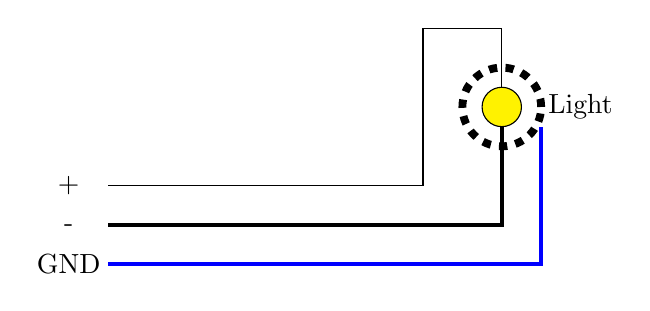
\begin{tikzpicture}
\draw [draw=blue, line width=0.5mm] (0,0) --(5.5,0)--(5.5,1.75) node(A){};
\draw [draw=black, line width=0.5mm] (0,.5)--(5,0.5)--(5,1.75);
\draw (0,1)--(4,1)--(4,3)--(5,3);
% (5,2); node[circle,radius=1cm,draw=black, line width=0.5 mm](L) {Light};
\draw (5,3)--(5,2.25);
\node[draw,circle,minimum size =0.5cm, fill=yellow] at (5,2){};
\node[draw,circle,minimum size =1cm, line width=1 mm, dashed] at (5,2){};
\node at (-.5,1) {+};
\node at (-.5,.5) {-};
\node at (-.5,0) {GND};
\node at (6,2) {Light};
\end{tikzpicture}
\caption{Light fixture showing ground wire protection. The dashed line represents the fixture's metal casing.}
\label{F:23P}
\end{center}
\end{figure}

Now consider these two situations, called case 1 and case 2.\par

\begin{itemize}
\item Case 1. The + and neutral (-) wires have rusted and broken off the light. The +wire now unintentionally touches the light's casing.
\item Case 2. The + and neutral (-) wires have rusted and broken off the light. The neutral (-) touches the light casing.
\end{itemize}

Consider case 1 with the + wire contacting the casing. If the casing is grounded via the extra wire (connected to the third prong), then as soon as the + wire comes into contact with the casing, a large current will flow from the + wire through the casing, then through the third wire and back to the breaker box. This current will likely exceed the 10 or 15A limit for the circuit breaker. This current will trip the breaker and shut off the circuit. By the time a person unwittingly touches the casing, the circuit should be disconnected and the person should be OK.\par

Of course, the light will no longer work and someone might notice. When the person tries to reset the breaker, the breaker should immediately re-trip, indicating a problem and potentially a hazard.\par

Consider the situations shown in Table~\ref{T:2P3}:\par
\begin{table}[H]
\begin{center}
\begin{tabular}{c|c|c|c}
two prong or three prong?&status&person touching casing&shock hazard?\\ \hline
2	&	no problem	& yes	& no\\ \hline
2	&	case 1		& no	& no\\ \hline
2	&	case 1		& yes	& \textbf{yes}\\ \hline
2	&	case 2		& yes	& no\\ \hline
3	&	no problem	& yes	& no\\ \hline
3	&	case 1		& no	& no\\ \hline
3	&	case 1		& yes	& no*\\ \hline
3	&	case 2		& yes	& no\\ \hline
\end{tabular}\par
\caption{Situations with 2-prong or 3-prong wiring}
\label{T:2P3}
\end{center}
\end{table}

\begin{blevel}
Draw a sketch like Figure~\ref{F:23P}, but for the situation occuring in row 7 of the table.
\end{blevel}
%%%%%%%%%%%%%%%%%%%%%%%%%%%%%%%%%%%%%%%%%%%%%%%%%%%%%%%%%%%%%%%%%%%%%%%
\section{Light-bulbs and LEDs}
A light-bulb or LED is a device that converts electrical energy into photons that are visible to the human eye. Older incandescent light bulbs operate by making a wire so hot that it glows white. This type of bulb wastes most of the energy as heat. Think of it like using a campfire to light up a living room.\par
Newer bulbs, like LEDs, more directly create photons and are much more efficient.

\begin{alevel}
What does LED stand for?
\end{alevel}

\begin{blevel}
What is a diode?
\end{blevel}

\begin{alevel}
At what temperature must something be in order to glow red? Look it up online.
\end{alevel}

%%%%%%%%%%%%%%%%%%%%%%%%%%%%%%%%%%%%%%%%%%%%%%%%%%%%%%%%%%%%%%%%%%%%%%%%%%%%
\section{Voltage sources}
A voltage source produces a constant voltage difference between two points, almost\footnote{It can't produce infinite current.} regardless of the amount of current that would be needed.
\par
Solar cells can be modeled as decent voltage sources because they produces roughly steady voltages but with variable amounts of current. More sunlight allows the panel to provide more current and therefore more power, but the voltage remains roughly the same.
\par
A wall socket also represents a fairly ideal voltage source, at least until the current exceeds the limit for the circuit breaker at which point the voltage goes to zero. Wall sockets in the US produce about 120 Volts AC, and provide close to the same voltage difference whether you draw 1 Amp of current or 10 Amps of current. 

\par
%%%%%%%%%%%%%%%%%%%%%%%%%%%%%%%%%%%%%%%%%%%%%%%%%%%%%%%%%%%%%%%%%%%%%%%%%%%%
\section{Current sources}
Current sources provide steady currents instead of steady voltages. The symbols for voltage sources and current sources are shown in Figure~\ref{F:2SCV}.
\par

\begin{figure}[H]
\begin{center}
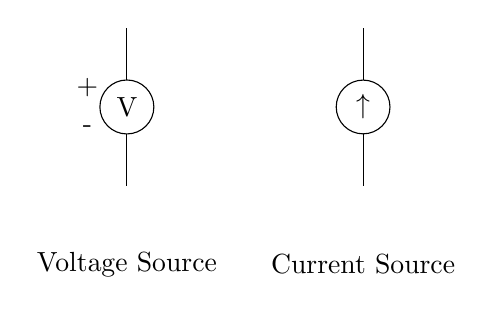
\begin{tikzpicture}
\node at (1,-1) {Voltage Source};
\node at (4,-1) {Current Source};
\draw (1,0)--(1,1) node[circle, draw=black, radius=1cm, fill=white]{V}--(1,2);
\node at (0.5,1.25) {+};
\node at (0.5,.75) {-};
\draw (4,0)--(4,1) node[circle, draw=black, radius=2cm, fill=white]{$\uparrow$}--(4,2);
\end{tikzpicture}
\caption{Symbols for voltage sources and current sources.}
\label{F:2SCV}
\end{center}
\end{figure}

Note the plus-minus indication on the voltage source, to show the more positive side. The current source arrow already shows the direction of the current. If the current source value were negative, then the current flows opposite the direction of the arrow.

\begin{alevel} A source produces the following combinations of voltage and current: {V=10V, I=3A} and  {V=9.9V, I=12A}. Is this source behaving more like a current source or a voltage source?
\end{alevel} 

\begin{blevel} A current source produces 10 Amps at a voltage of 5V. If the voltage were doubled, what would likely happen to the current being produced?
\end{blevel} 

%%%%%%%%%%%%%%%%%%%%%%%%%%%%%%%%%%%%%%%%%%%%%%%%%%%%%%%%%%%%%%%%%%%%%%%%%%%%
\section{Resistors}
Resistors are electrical components that hinder or \emph{resist} the flow of current. It takes effort (energy) to push charge through a resistor. The more charge per second you need to get through the resistor, the more energy (effort) it will take.\par

Sometimes, resistors are added intentionally, other times, the natural resistance of a component or wire is modeled as a resistor.\par
\par
\begin{alevel}
What is another name for energy per charge?
\end{alevel}

For some objects, like a typical chunk of metal, the flow (current) varies roughly proportionally to the change in the voltage across it. This is captured by something called Ohm's Law.
\par
\begin{align*}
\Delta V \sim I	&&\text{Ohm's Law}
\end{align*}

The proportionality constant can be written as R.\par
\begin{align}
\Delta V = IR	&&\text{Ohm's Law}
\end{align}
 Note: the $\Delta$ on the $\Delta V$ is often omitted because it is usually obvious that you're referring to a change in voltage, and not some meaningless absolute voltage with respect to who-knows-what reference point. \par

\begin{alevel}
What is the standard S.I. unit of resistance?
\end{alevel}

\begin{clevel}
In terms of Coulombs, seconds, and Joules, what are the units of resistance?
\end{clevel}

\begin{clevel}
In terms of Coulombs, seconds, meters, and kg, what are the units of resistance? Hint: What is a Joule?
\end{clevel}

For better or worse, Ohm's law is NOT some fundamental relationship that is true all the time. Instead, it is only sort-of true some of the time. People design manufactured resistors, like the ones in the lab, to mimic Ohm's Law pretty well. But other devices, like LEDs, do not much behave this way at all\footnote{LEDs are better modeled as a voltage source. Or better yet, as a voltage source in series with a resistor.}\par

\begin{blevel}
Which of the following formulae are perfectly accurate (either because it's a definition or because it describes a model that has not (yet) been contradicted by experiment) verses a approximate model (engineering hack) that we know is not exactly right?\\
\begin{center}
\begin{tabular}{|c|c|}\hline
equation & (always correct) or (hack)? \\ \hline
$F_f=\mu F_N$ & \\ \hline
$V=IR$ & \\ \hline
$\rho=\frac{mass}{Vol}$ & \\ \hline
$PV=nRT$ & \\ \hline
\end{tabular}
\end{center}
\end{blevel}

Resistors on a diagram are drawn with a zig-zag line. Figure~\ref{F:21} shows a current source connected to a $5 \Omega$ resistor.

\begin{figure}[H]
\begin{center}
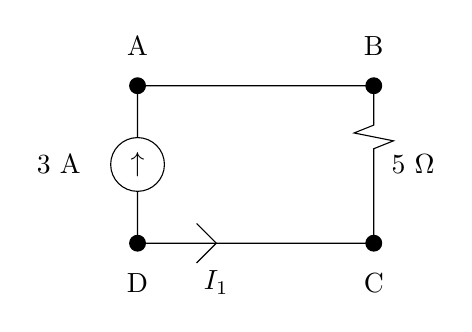
\begin{tikzpicture}
\draw (1,0)--(1,1) node[circle, draw=black, radius=2cm, fill=white]{$\uparrow$}--(1,2)--(4,2)--(4,1.5)--(3.75,1.4)--(4.25,1.3)--(4,1.2)--(4,0)--(1,0);
\node at (0,1) {3 A};
\node at (4.5,1) {5 $\Omega$};
\filldraw (1,2) circle[radius=1 mm];
\node at (1,2.5) {A};
\filldraw (4,2) circle[radius=1 mm];
\node at (4,2.5) {B};
\filldraw (4,0) circle[radius=1 mm];
\node at (4,-.5) {C};
\filldraw (1,0) circle[radius=1 mm];
\node at (1,-.5) {D};
\draw (1.75,.25)--(2,0)--(1.75,-.25);
\node at (2,-.5) {$I_1$};
\end{tikzpicture}
\caption{A current source connected to a resistor. Note how current $I_1$ is labeled with an arrow.}
\label{F:21}
\end{center}
\end{figure}

\begin{blevel}
Fill in Table~\ref{T:21}.
\end{blevel}

\begin{table}[H]
\begin{center}
\begin{tabular}{|c|c|c|}\hline
item&answer&hints\\ \hline
$I_1$	&	&	\\ \hline
$V_{AB}$	&	&	\\ \hline
$V_{BC}$	&	& use Ohm's law	\\ \hline
$V_{AD}$	&	&	\\ \hline
$I_{from B to C}$	&	&	\\ \hline
Power absorbed by R	&	& use equation ~\eqref{eq:PIV}	\\ \hline
Power produced by current source	&	&	\\ \hline
\end{tabular}
\label{T:21}
\caption{Summary of select parameters for simple circuit.}
\end{center}
\end{table}

One can connect resistance (an extrinsic property) to resistivity (an intrinsic property). \footnote{An \textbf{extrinsic} property depends on something's amount or shape. An \textbf{intrinsic} property does not depend on how much of it you have. Density is an intrinsic property whereas mass is not.}\par

\begin{align}
R = \rho \frac{L}{A} \label{eq:2rho}
\end{align}
Where $\rho$ is the resistivity of the material, L is its length and A is its cross-sectional area.

\begin{blevel}
Determine the resistance of a 20 m long section of 12 gauge copper wire. Hint: look up the radius of 12 gauge wire. 12-gauge wire is typical for household wiring.
\end{blevel}

\begin{blevel}
An aluminum wire inside a computer chip carries a signal from one side of the chip to the other. The dimensions of the wire are 5 mm by 1 micron by 0.1 micron. What is the resistance of the wire? If 100mA of current pass through the wire, what is the voltage dropped across it? How much power is dissipated by the wire? 
\end{blevel}

\begin{dlevel}
Continuing the previous problem. If the heat had nowhere to go but to heat up the Al wire, how much would the temperature of the wire increase after 1 minute? How much time until the wire melted?
\end{dlevel}

\subsection{Analog of current with heat flow}
We can substitute Equation~\eqref{eq:2rho} expression for resistance into Ohm's law and come up with an equation for electricity flow that is very similar to the flow of heat.

\begin{align*}
I = \frac{\Delta V}{R}	\\
\frac{dq}{dt} = \frac{\Delta V}{\rho}\frac{A}{L}=(\frac{1}{\rho})\frac{A\Delta V}{L}&&	\text{``electricity flow" equation}\\
\frac{dQ}{dt}=	\frac{kA\Delta T}{L}&&				\text{heat flow equation}
\end{align*}
What drives heat to flow from one side of a material to the other? Answer: a temperature difference. What drives electrical charge to flow from one side of a material to the other? Answer: a voltage difference.

\begin{blevel}
A 0.5 meter long section of 12-gauge Cu wire connects between the inside of a house ($65^0 F$) and the outside of a house ($35^0 F$). How many Joules of heat flow out of the house through the wire in one minute?
\end{blevel}

\begin{blevel}
A 0.5 meter long section of 12-gauge Cu wire connects between one side of a 9V battery and the other. How many Coulombs of charge flow along the wire in one minute?
\end{blevel}



